% 2006_liaoning_liberal_q15_fig1: hemisphere with inscribed hexagonal pyramid P-ABCDEF
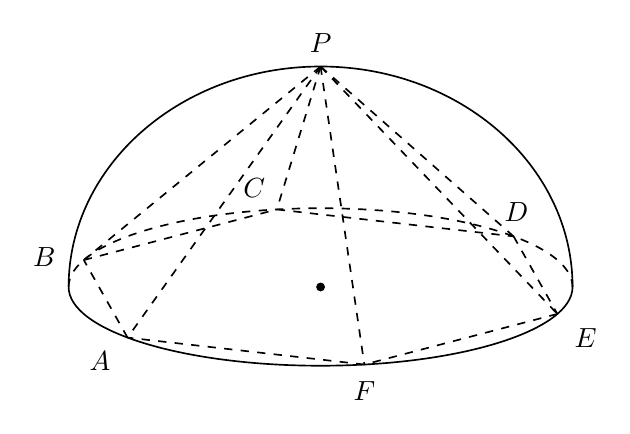
\begin{tikzpicture}[x=1cm,y=1cm,font=\normalsize,
  geometry edge/.style={solid,line width=.6pt},
  geometry label/.style={font=\normalsize,inner sep=2pt}]
% dome and rim: dome rx=3.2 ry=2.8, base ellipse rx=3.2 ry=1.0 at y=0
% outer dome (solid)
\draw[geometry edge] (-3.2,0) arc (180:0:3.2 and 2.8);
% front rim (solid)
\draw[geometry edge] (-3.2,0) arc (180:360:3.2 and 1.0);
% back rim (dashed, hidden)
\draw[geometry edge,dashed] (-3.2,0) arc (180:0:3.2 and 1.0);
% hexagonal base vertices on ellipse R=2.8,r=0.9
\coordinate (P) at (0,2.8);
\coordinate (A) at (-2.4513422180,-0.6427876097);
\coordinate (B) at (-3.0070163865,0.3420201433);
\coordinate (C) at (-0.5556741685,0.9848077530);
\coordinate (D) at (2.4513422180,0.6427876097);
\coordinate (E) at (3.0070163865,-0.3420201433);
\coordinate (F) at (0.5556741685,-0.9848077530);
\coordinate (Odot) at (0,0);
% lateral edges P to vertices (all dashed, interior)
\draw[geometry edge,dashed] (P)--(A);
\draw[geometry edge,dashed] (P)--(B);
\draw[geometry edge,dashed] (P)--(C);
\draw[geometry edge,dashed] (P)--(D);
\draw[geometry edge,dashed] (P)--(E);
\draw[geometry edge,dashed] (P)--(F);
% hexagonal base perimeter (all dashed interior to match original)
\draw[geometry edge,dashed] (A)--(B);
\draw[geometry edge,dashed] (B)--(C);
\draw[geometry edge,dashed] (C)--(D);
\draw[geometry edge,dashed] (D)--(E);
\draw[geometry edge,dashed] (E)--(F);
\draw[geometry edge,dashed] (F)--(A);
% sphere centre dot
\fill (Odot) circle (1.6pt);
% labels offset from strokes
\node[geometry label,above] at (P) [yshift=3pt] {$P$};
\node[geometry label,below left] at (A) [xshift=-4pt,yshift=-3pt] {$A$};
\node[geometry label,left] at (B) [xshift=-8pt,yshift=1pt] {$B$};
\node[geometry label,above left=2pt] at (C) {$C$};
\node[geometry label,above=2pt,xshift=1pt,yshift=1pt] at (D) {$D$};
\node[geometry label,below right] at (E) [xshift=4pt,yshift=-3pt] {$E$};
\node[geometry label,below] at (F) [yshift=-4pt] {$F$};
\end{tikzpicture}
